\documentclass{article}
\usepackage{amsmath,amssymb}
\usepackage{hyperref}
\usepackage{graphicx}
\usepackage{todonotes}

\title{\bf{Laboratory Project Two: Calibration of an Orifice Meter}}
\author{Nicholas Malaya \\ Department of Mechanical Engineering \\
University of Texas at Austin} \date{} 

\begin{document}
\maketitle
\date{}
\newpage
\section{Objectives}

\textbf{A short paragraph listing the specific objectives of this laboratory.}   

I believe the purpose of this laboratory was to learn about
several of the considerations necessary to properly operate an
LDV. Unlike the previous labs, the LDV had quite a bit of operational
details required to even begin gathering data. Our group took over an
hour to first start up the laser, play around with the oscilloscope,
etc. 

Beyond a familiarity with the LDV apparatus, this is also the first lab
where we have attempted to gather spatially resolved measurements. In
particular, we have characterized the free-stream turbulence (which we
expect to be statistically spatially independent) as well as the flow in
the wake of a cylinder. 

Common with the previous efforts, this work was also focused on
estimating the uncertainties (and ultimately, plausibility ) of our
measurements, both through uncertainty estimates as well as comparing
with available results in the literature. 

It was also my favorite lab. Felt very high tech. 

\section{Background and Experimental Details}

\textbf{Describe the basic operation of an LDV.}

I see the LDV as a four step process. 

\begin{itemize}
 \item Laser Crossing
 \item Particle movement through the fringes
 \item Light collected
 \item Postprocessing
\end{itemize}

Two laser beams cross, creating an interference pattern.\todo{finish me}


\textbf{Explain what frequency
shifting is, and why it is used. Calculate the following: 
\begin{itemize}
 \item Size of the Probe Volume
 \item Expected frequency response of the glass sphere seed particles
\end{itemize}
}   

We use frequency shifting so that we can measure flow reversals.\todo{expand}

The size of the probe volume is given by Stavros on page 267, 
\begin{equation}
 V_p = \frac{\pi d_{fe}^3}{6\text{Cos}(\theta/2)\text{Sin}(\theta/2)}
\end{equation}

% the doppler frequency of the particle is the normal velocity over the
% fringe spacing, which was: X-direction: 3.744um; y-direction: 3.551um
% (taken from Flowsizer) 

  % \begin{figure}[!htb]
  %  \begin{center}
  %   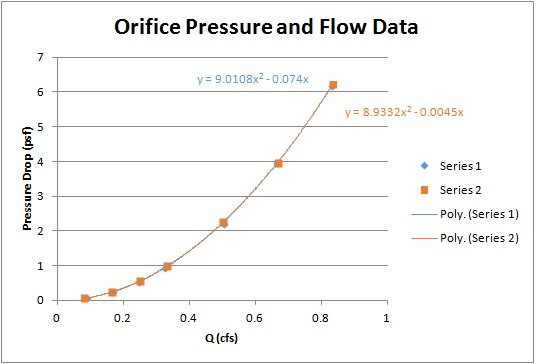
\includegraphics[width = 12 cm]{figs/Q_dP_fits.jpg}
  %   \caption{A plot of repeatability of the experiment. }
  %   \label{orif-zoom}
  %  \end{center}
  % \end{figure}

\section{Experiment One: Freestream}

\textbf{Indicate the frequency shift and bandpass filter settings used,
and why.} 

\section{Experiment Two: Wake Measurements}

\textbf{Present results from your wake measurements, including
uncertainty of the measurements. Compare your results with data in the
literature and comment on similarities and differences. } 


\section{Conclusions}


\textbf{Conclude by giving your opinion about whether your measurements
are more or less reliable than measurements in the literature.} 

%
%
%
\end{document}

% LocalWords:  reynolds H20 piecewise RDG yar
